Transformational music theory is a way to analyse music by focusing on the transformations between musical object rather than on the objects themselves. It was mainly developped by David Lewins in 1980's \cite{rahn_lewin_1987}. His work relied on algebra, and particularly on group theory. Indeed, by using well temperament, we obtain a 12 element dodecahedron, with each vertex corresponding to one of the 12 semi-tones. Each vertex of this dodecahedron is called a \textbf{pitch class}(see Figure\ref{fig:dode-id}).

There are then 12 rotational symmetries and 12 axial symmetries of this dodecahedron (called  respectively \textbf{transpositions} and \textbf{inversions} and written $T_i$\label{nomencl:Ti} (see Figure \ref{fig:dode-T2}) and $I_i$\label{nomencl:Ii} (see Figure \ref{fig:dode-I4}) for $i\in [\![1,12]\!]$ by music theorists). If we only consider the transpositions, we actually a group isomorphic to the group $\mathbb{Z}_{12}$\label{nomencl:Zn}. The group composed of composed of the transpositions and the inversions is well known by mathematicians as the dihedral group but called by musicologists
$T/I$ \label{nomencl:TI} (see Figure \ref{fig:dode-TI}).

\begin{figure}[ht]
    \begin{subfigure}{.29\textwidth}
        \centering
        \newcounter{itemcount}
        \setcounter{itemcount}{450}
        \renewcommand*{\do}[1]{
            \filldraw [black](\number\value{itemcount}:3cm)
            circle (1.5pt)
            node[anchor={\number\value{itemcount}-180}]
                {#1\addtocounter{itemcount}{-30}};}
        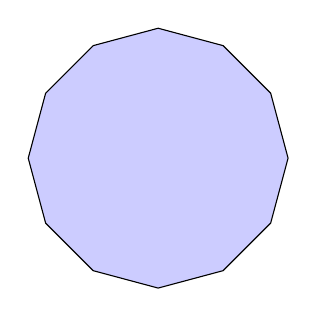
\begin{tikzpicture}[scale=0.55]
            \dolistloop{\pc}
            \draw[fill=blue!20] (90:3cm) -- (60:3cm) -- (30:3cm) -- (0:3cm) --  (330:3cm) -- (300:3cm) -- (270:3cm) -- (240:3cm) -- (210:3cm) -- (180 :3cm) -- (150:3cm) -- (120:3cm) -- cycle;
        \end{tikzpicture}
        \caption{The 12 pitch-classes dodecahedron}
        \label{fig:dode-id}
    \end{subfigure}%
    {\LARGE$\xRightarrow{T_2}$}%
    \begin{subfigure}{.3\textwidth}
        \centering
        \setcounter{itemcount}{510}
        \renewcommand*{\do}[1]{
            \filldraw [black](\number\value{itemcount}:3cm)
            circle (1.5pt)
            node[anchor={\number\value{itemcount}-180}]
                {#1\addtocounter{itemcount}{-30}};}
        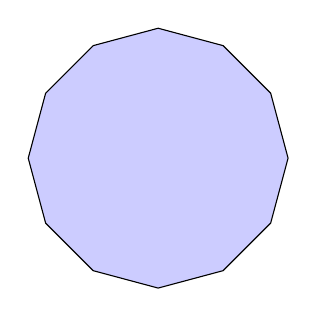
\begin{tikzpicture}[scale=0.55]
            \dolistloop{\pc}
            \draw[fill=blue!20] (90:3cm) -- (60:3cm) -- (30:3cm) -- (0:3cm) --  (330:3cm) -- (300:3cm) -- (270:3cm) -- (240:3cm) -- (210:3cm) -- (180 :3cm) -- (150:3cm) -- (120:3cm) -- cycle;
        \end{tikzpicture}
        \caption{Transposition of 2 semi-tones (Rotation)}
        \label{fig:dode-T2}
    \end{subfigure}%
    {\LARGE$\xRightarrow{I_4}$}%
    \begin{subfigure}{.3\textwidth}
        \centering
        \setcounter{itemcount}{510}
        \renewcommand*{\do}[1]{
            \filldraw [black](\number\value{itemcount}:3cm)
            circle (1.5pt)
            node[anchor={\number\value{itemcount}-180}]
                {#1\addtocounter{itemcount}{30}};}
        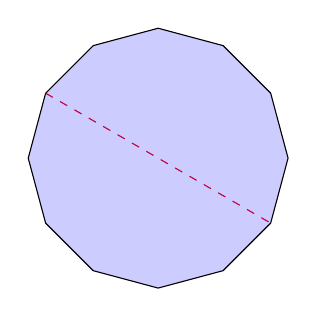
\begin{tikzpicture}[scale=0.55]

            \dolistloop{\pc}
            \draw[fill=blue!20] (90:3cm) -- (60:3cm) -- (30:3cm) -- (0:3cm) --  (330:3cm) -- (300:3cm) -- (270:3cm) -- (240:3cm) -- (210:3cm) -- (180 :3cm) -- (150:3cm) -- (120:3cm) -- cycle;
            \draw[purple,dashed] (150:3cm) -- (330:3cm);
        \end{tikzpicture}
        \caption{$4^{th}$ inversion  (Symmetry)}
        \label{fig:dode-I4}
    \end{subfigure}%
    \caption{Transpositions and inversions in a dodecahedron}
    \label{fig:dode-TI}
\end{figure}


This $T/I$ paradigm could then be applied to musical object. Indeed, we can represent a C major chord (see Figure \ref{fig:Cmajor}) inside the dodecahedron (to make the figure more readable, we changed the dodecahedron into a circle).
\newcounter{itemcount2}
\setcounter{itemcount2}{450}
\renewcommand*{\do}[1]{
    \filldraw [black](\number\value{itemcount2}:3cm)
    circle (1.5pt)
    node[anchor={\number\value{itemcount2}-180}]
        {#1\addtocounter{itemcount2}{-30}};}

\begin{tzfigure}{
        \caption{The C Major chord in the chromatic circle}
        \label{fig:Cmajor}
    }
    \dolistloop{\pc}
    \draw[fill=blue!20] (90:3cm) -- (330:3cm) -- (240:3cm) -- cycle;
    \draw [domain=0:360,samples=60] plot ({3*cos(\x)}, {3*sin(\x)});
\end{tzfigure}




The intuition of Allen Forte was that instead of considering triads (three notes chord) as the set of the notes that compose them, we should consider them as the set of the intervals between each note. As a result, every inversion of chord \footnote{the term inversion has to be taken here from a musical point of view, for instance the inversions of a C major chord are C-E-G, G-C-E, E-G-C. Later in this report, we will use inversion as a member of the $T/I$ group and we will stick to it} will be in the same \textbf{pitch-class set}\cite{forte_1980}. This can be seen in the geometrical point of view where the simple fact  of representing the chord as a triangle allow to forget any order between the three note. Similarly, all the transpositions of the chord will be in the same pitch-class.


\section{Presentation of Klumpenhouwer's networks}
Klumpenhouwer networks, or K-nets, were then introduced by Henry Klumpenhouwer, former PhD student of Lewin, to formalize the relation between two chords\cite{lewin_1990}.

The idea behind K-nets is that instead of analyse chords transformations threw transposition only, which is not very rich, we could use also inversions.

\begin{defn}
    A Klumpenhouwer network is a graph (also called a network) where objects are pitch classes and arrows between objects are labeled by an element of the group $T/I$.
\end{defn}

\begin{defn}
    Two K-nets $K$ and $K'$ are said \textbf{isographic} if and only if :
    \begin{itemize}
        \item there exist a bijection $f:V(K)\rightarrow V(K')$ from the set of vertices $V(K)$ to $V(K')$
        \item if there is an arrow $a:s\rightarrow t$ where $s,t\in V(K)$ in $K$, then there is an arrow $a':f(s)\rightarrow f(t)$ in $K'$
        \item there is an automorphism $F \in Aut(T/I)$\label{nomencl:Aut} such that if $X$ is the label of an arrow $a:s\rightarrow t$, then $F(X)$ is the label of the arrow $a':f(s)\rightarrow f(t)$.
    \end{itemize}
\end{defn}

\begin{prop}[\cite{lewin_1990}]
    The T/I automorphisms are exactly the $F\big<u,j\big>$ such that $u\in\{1,5,7,11\}$ and $j\in\mathbb{Z}_{12}$ where
    \begin{align*}
        F\big<u,j\big>(T_n) & = T_{un}   \\
        F\big<u,j\big>(I_n) & = I_{un+j}
    \end{align*}
\end{prop}


\begin{note}
    The T/I automorphisms such that $u = 1$ (resp. $u = 11$) are called \textbf{positive automorphisms} (resp. \textbf{negative automorphisms}).
\end{note}


\begin{exmp}
    To represent a triad, Klumpenhouwer uses 3 pitch classes and 3 arrows of the form we can see in Figure \ref{fig:KCmajor}.
    Geometrically, we can see in Figure \ref{fig:Rtransf} that the inversion $I_4$ would transform our C major triangle into a A minor triangle (we swap C and E and G becomes A).
    \begin{tzfigure}{
            \caption{The $I_4$ inversion on the C major chord}
            \label{fig:Rtransf}
        }
        \dolistloop{\pc}
        \draw[fill=purple!20,opacity=0.7] (90:3cm) -- (330:3cm) -- (180:3cm) -- cycle;
        \draw[fill=blue!55, fill opacity=0.6] (90:3cm) -- (330:3cm) -- (240:3cm) -- cycle;
        \draw (90:3cm) -- (330:3cm) -- (240:3cm) -- cycle;
        \draw [dashed, thick, purple, opacity=1] (30:3cm) -- (210:3cm);
        \draw [domain=0:360,samples=60] plot ({3*cos(\x)}, {3*sin(\x)});
    \end{tzfigure}

    Actually, positive (resp. negative) isographies and transposition  (resp. inversions) are in one to one correspondance :
    \begin{align*}
        T_j & \mapsto F(1,j)  \\
        I_j & \mapsto F(11,j) \\
    \end{align*}
    This correspondance might seem hazardous but we will see that in EK-paradigm it is extremely accurate. If we follow this corresponence, we get an isography between two K-nets representing respectively C major and A minor (see Figure \ref{fig:Kisography}).
    \begin{figure}[h]

        \begin{subfigure}{.29\textwidth}
            \centering            
            \begin{tikzpicture}
                % https://tikzcd.yichuanshen.de/#N4Igdg9gJgpgziAXAbVABwnAlgFyxMJZABgBoAmAXVJADcBDAGwFcYkQBhEAX1PU1z5CKMgEZqdJq3YBRHnxAZseAkTLEJDFm0QgA4jwkwoAc3hFQAMwBOEALZIyIHBCSiaAIxhgoSAMxOWtK6ACoA+gAs8la2Dojuzq6I5J7evogBNEE6IOF+0SA29o40LkgpIF4+SAC0mc70WIzskGBsNHAAFliWOCUgjPRejAAKAirCINZYJp19WVI5AJJhAOyG3EA
                \node[scale=1.3] (a) at (0,0){
                \begin{tikzcd}
                    G                                                            \\
                    E \arrow[u, "T_3", bend left]                                \\
                    C \arrow[u, "T_4", bend left] \arrow[uu, "I_7"',leftrightarrow,  bend right]
                \end{tikzcd}
                };
            \end{tikzpicture}
                        \caption{A Klumpenhouwer network for the C major chord}
            \label{fig:KCmajor}
        \end{subfigure}%
        {\LARGE$\xRightarrow{F\big<11,4\big>}$}%
        \begin{subfigure}{.29\textwidth}
            \centering
           
            \begin{tikzpicture}

                % https://tikzcd.yichuanshen.de/#N4Igdg9gJgpgziAXAbVABwnAlgFyxMJZABgBoAmAXVJADcBDAGwFcYkQBhEAX1PU1z5CKMgEZqdJq3YBRHnxAZseAkTLEJDFm0QgA4jwkwoAc3hFQAMwBOEALZIyIHBCSiaAIxhgoSAMxOWtK6ACoA+gAs8la2Dojuzq6I5J7evogBNEE6IOF+0SA29o40LkgpIF4+SAC0mc70WIzskGBsNHAAFliWOCUgjPRejAAKAirCINZYJp19WVI5AJJhAOyG3EA
                \node[scale=1.3] (a) at (0,0){
                \begin{tikzcd}
                    A                                                            \\
                    C \arrow[u, "T_9", bend left]                                \\
                    E \arrow[u, "T_8", bend left] \arrow[uu, "I_2"',leftrightarrow,  bend right]
                \end{tikzcd}
                };
            \end{tikzpicture}
            \caption{A Klumpenhouwer network for A minor chord}
            \label{fig:KAminor}
        \end{subfigure}
        \caption{C major and A minor are isogrphic}
        \label{fig:Kisography}
    \end{figure}
\end{exmp}




\section{Presentation of PK-nets}
Klumpenhouwer networks propose many ways to analyse music but they do not allow to compare graphs of different form : if we want to compare a 3-note and a 4-note chord, there is no way there is an isography between K-nets representing them.

PK-nets\cite{PAAE2016} where introduced by Alexandre Popoff in 2015\cite{popoff2015categorical} and are a generalization of K-nets that allows comparison between any type of objects. They are defined in the paradigm of category theory. Let's first present informally category theory.

A category is a particular case of multigraph (i.e. a graph where there can be multiple arrows between to vertices), which means we are not so far from Klumpenhouwer's concept. However, one of the main goal of representing threw mathematics is to point some patterns or ways of construction usually used in music creation. So we would like to have a general enough mathematic construction so it encompasses as many musical concepts possible but restricted enough so that we are not overwhelmed by too many possible interpretation of the same piece of music.

In fact categories are one of the best framework to get a structured system without losing too many generalities.
One of the more important concept behind category theory is compositionality. Musically, it also seems a basic concept : if I can go from $C$ to $D$ and from $D$ to $E$, I would expect I can go from $C$ to $E$. This is in fact the whole concept of a scale : if from $C$, I can hit $D$, $E$, $F$, $G$, $A$, $B$ and finally to $C$ again, then, implicitely, I can go from any of the pitchs of the scale to another pitch of the scale.

A category is in fact a graph such that the composition of two arrows always exists and that for each vertex (called an object in category theory), there is an arrow on itself called the identity of this object. This is a minimal structure that we want to use to go further than the K-net analysis.

\begin{defn}\textbf{Set}\label{nomencl:Set} is the category where objects are the sets and morphisms are functions between sets.
\end{defn}

This is a non trivial definition, because we could face the Russell paradox. We will not go deeper in size problems in category. We will just point at the fact that we might have problem of size at some points.


The idea behind PK-nets is to lean on the category $\bf Set$ in such a way that musical objects are sets and relation between them are arrows. However, we need to add a frame to this principle. First of all, if we use the example of K-nets, we would like to use the group T/I to act on a 12 elements set. In fact, a group can be defined as a single-object category where the elements of the group are the reflexive arrows of this object and the group operation corresponds to the composition of two arrows.

The group action can be defined as a functor between the category T/I and the category $\bf Set$ which associates the unique object of T/I to a 12 elements set and the arrows to functions on this set. Indeed, functors in category theory are defined in such a way that they preserve identity and compositions, which makes every functor from a group to $\bf Set$ an action of this group on some set. So we have defined the set of pitch classes and how we want to analyse it.

We still need to know how to select some sets to be musical objects to analyse. For this, we use a category $\Delta$ where every object of $\Delta$ represents a musical object and the arrows between them their interactions. We then send  $\Delta$ on $\bf Set$ via a functor $R$ to have knowledge about the components of each musical object. But these interactions between objects are not defined either. So we need also a functor $F$ from $\Delta$ to $T/I$ which will exhibit how musical objects are related to each other.

To finish, we need to send each musical object seen as a set to the set of pitch-classes. This is the role of the natural transformation $\phi$. More formally,  as


\begin{defn}[PK-net\cite{popoff2015categorical}]
    \label{def:pk-net}
    For any category $\mathcal{C}$ and any functor $S:\mathcal{C} \rightarrow \Delta$ with non empty values (i.e. $\forall c \in \mathcal{C}, S(c) \neq \emptyset$), we can define a PK-net as follow :

    Let $\Delta$ be a small category and $R : \Delta \rightarrow \bf Set$ a functor with non empty values. Then a \textbf{PK-net} of form $R$ and with support $S$ is a tuple $\big<R,S,F,\phi\big>$ where $\phi : R \rightarrow SF$ is a natural transformation from $R$ to $SF$ (see Figure\ref{fig:PK-definition})

    \begin{tzcategory}{\caption{PK-net definition}
            \label{fig:PK-definition}}
        \node[scale=1.3] (a) at (0,0){
            \begin{tikzcd}[column sep=tiny]
                \Delta
                \ar[ddr, "R"',""{name=R,right}]
                \ar[rr,"F"]
                & &
                \mathcal{C}
                \ar[ddl,"S",""{name=S,left}] \\
                & \ar[Rightarrow,bend left=80,from=R, to=S, "\phi"']& \\
                & \bf Set &
            \end{tikzcd}
        };
    \end{tzcategory}

\end{defn}

As in the K-nets definition, we would like to transform a PK-net into another. However, we are forced here to have composition between homographies, since we are in a categorical paradigm.


\begin{defn}[Category of PK-nets\cite{popoff2015categorical}]
    For a fixed functor $R: \Delta \rightarrow \bf Set$, we can define the category $ \text{PKN}_R$ of PK-nets of form $R$ such that :
    \begin{itemize}
        \item the objects of $\text{PKN}_R$\label{nomencl:PKNR} are the PK-nets $\big<R,S,F,\phi\big>$ as defined in Definition \ref{def:pk-net}
        \item the morphisms between $\big<R,S,F,\phi\big>$ and $\big<R,S',F',\phi'\big>$ are pairs $\big< N,\nu\big>$ such that $N : \mathcal{C} \rightarrow \mathcal{C}'$ is a functor and $\nu : S \rightarrow S'N$ is a natural transfomation such that $\phi' = (\nu F)\circ \phi$.
    \end{itemize}
\end{defn}

\begin{note}
    The morphisms between PK-nets are called \textbf{PK-homographies}.
\end{note}




